\section{Motivations}
\subsection{Fallacy: LBA-based lifetime prediction}

Current automatic methods predict the lifetime of data based on the update
frequency of LBAs~\cite{}.  For example, AutoStream~\cite{} assumes that, if
some LBAs are frequently rewritten by applications, those LBAs hold hot data.
This LBA-based lifetime prediction works poorly on modern applications, where
the majority of new data are written in an append-only manner.  To understand
the correlation between LBAs and the lifetime of data under append-only
workloads, we analyzed the write pattern of RocksDB~\cite{}, which is a
popular key-value store based on the LSM-tree algorithm~\cite{}.

Figure~\ref{fig:lba_lifetime}(a) shows the lifetime distribution of data
according to LBAs. Here, the lifetime of data is defined to be an elapsed time
(unit: $\mu$sec) from when it is newly written to a certain LBA to when it is
invalidated by an overwrite or a TRIM command. As shown in
Figure~\ref{fig:lba_lifetime}(a), there is no strong correlation between the
lifetime and LBAs -- all the data have very different lifetimes, regardless of
their LBA numbers. We also observed how the lifetimes of LBAs changed according
to the time in a more microscopic view.  For a small number of consecutive LBAs
(256 LBAs)\textcolor{red}{, composing a 1 MB chunk (Q: why should it be a chunk
not few LBAs?)}, we plot the trend of the lifetime of the chunk for 600 seconds
in Figure~\ref{fig:lba_lifetime}(b). As shown in the figure, the LBAs belonging
to the chunk first hold hot data. For example, at the logical time
\textcolor{red}{XX}, the lifetime of the chunk is close to \textcolor{red}{XX
$\mu$sec}.  At \textcolor{red}{YY}, however, its lifetime increases to
\textcolor{red}{XX $\mu$sec}. Then, the lifetime drops to \textcolor{red}{XX
$\mu$sec} at \textcolor{red}{XX}.  Consequently, our observations shown in
Figure~\ref{fig:lba_lifetime} indicate that, under append-only
workloads, LBAs couldn't be a useful metric that decides the hotness or
lifetime of data that they hold.

\begin{figure}[t]
	\centering
	\subfloat[Lifetime by address]{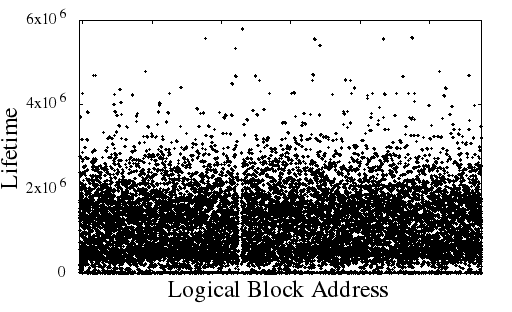
\includegraphics[width=0.25\textwidth]{figure/lba_lifetime}}
	\subfloat[Lifetime by time]{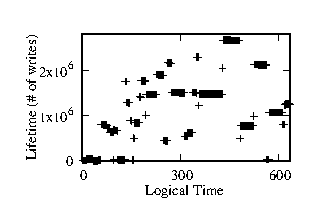
\includegraphics[width=0.22\textwidth]{figure/lifetime_in_chunk}}
	%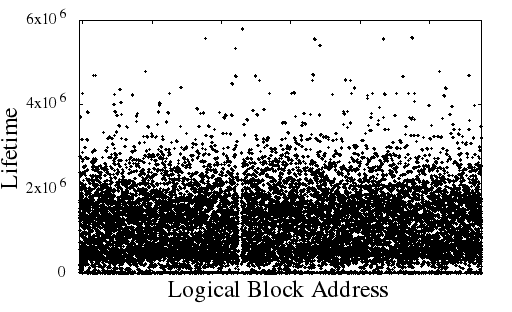
\includegraphics[width=0.9\linewidth]{figure/lba_lifetime} 
	\vspace{-10pt}
	\caption{
		The lifetime distribution according to the address and time.
		\textcolor{red}{(TODO: 1) it would be good to include same graphs with
		in-place update workloads; 2) add a unit in the y-axis.)}}
		\label{fig:lba_lifetime}
	\vspace{-15pt}
\end{figure}

%The address-based approach can not properly distinguishes the lifetime of the data written by
%the append-only workload.
%To sum up, although the application knows the lifetime of the written data, it is hard to 
%deliver the information to the system layer without modification.

\subsection{Program context as a lifetime predictor}
The lifetime of the data depends on the purpose of the application. 
In general, the writes for different purposes are implemented to have different execution paths.
For example, RocksDB writes a log file and a compaction file in a different functions.

The program context is defined by the summing instruction counter values 
of each execution path of function calls that lead to a write system call which causes write requests,
so it is useful for identifying the purpose of the application. 
Ha et al.~\cite{PCHa} proposed update time based data separator using PC. 
They predicted data update times by exploiting program contexts as hints. 
Since a program context represents a program phase and the same phase is likely to be executed multiple times, 
program contexts have been used in predicting future behavior of programs. 
We extend this approach to differentiate the lifetime of data through invalid time as well as update time. 
In particular, since append-only workloads such as RocksDB have a write-TRIM-write pattern, 
it is necessary to consider an invalid time for an accurate lifetime evaluation.
In previous studies~\cite{MultiStream}, especially for NoSQL DB workload, 
it is known that the lifetime of data can be distinguished by the behavior of applications such as logging, 
flushing, and compaction. 

\begin{figure}[!t]
\centering
\hspace{1pt}
\subfloat[manual: log]{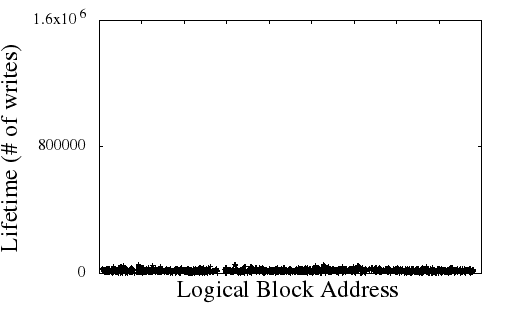
\includegraphics[width=0.23\textwidth]{figure/type_1}}
\subfloat[PC\#2]{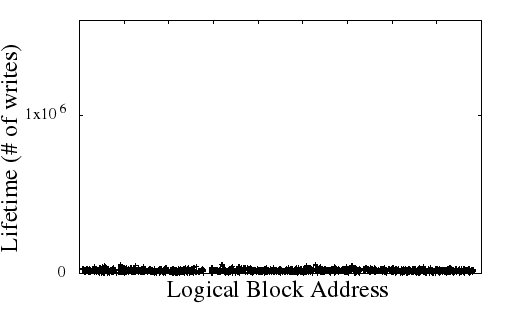
\includegraphics[width=0.23\textwidth]{figure/pcID_2}}
\hfill
\vspace{-10pt}
\subfloat[manual: flush] {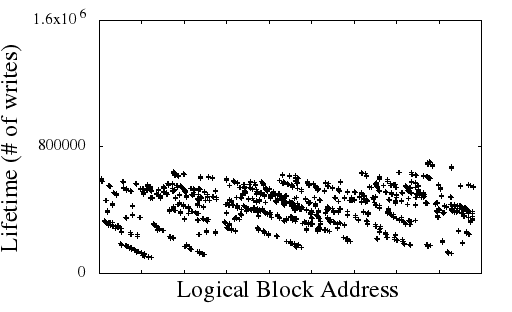
\includegraphics[width=0.23\textwidth]{figure/type_3}}
\subfloat[PC\#3]{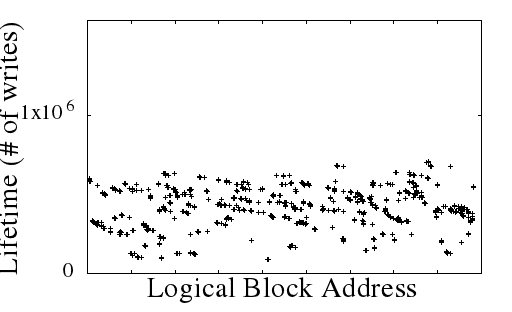
\includegraphics[width=0.23\textwidth]{figure/pcID_3}}
\caption{Data lifetime distributions of different PCs.} \label{fig:types_and_PCs}
\vspace{-20pt}
\end{figure}

In order to verify that the PC information is enough to recognize the behavior of these applications, 
we ran RocksDB and compared the data lifetimes when the type of data was manually identified 
aginst when the data is identified by PC values.
Figure~\ref{fig:types_and_PCs} shows the lifetime distribution of data separated by manual scheme and 
PC values for two cases, i.e., log and flush.
First, Figure~\ref{fig:types_and_PCs}(a) represents the lifetime of the log file of RocksDB. 
RocksDB's log data is short-lived because the data in memory is temporarily maintained
until the data is flushed to the storage for the consistency reason~\cite{RocksDB}.
Figure~\ref{fig:types_and_PCs}(b) depicts the data lifetime of ID 2 among the classified PCs 
according to the our proposed collection method.
As these two graphs have the same lifetime pattern, we can say PC ID 2 represents the context of the log file.
Similary, Figure~\ref{fig:types_and_PCs}(c) shows the lifetime of flushed static sorted table (SST)
files of RocksDB.
The flush operation stores the memory data as an SST file at level 0 of the LSM tree in the storage.
The file is deleted by a compaction operation that removes invalid data when each level is full.
Due to the characteristics of the LSM tree, which becomes smaller as it goes to top level,
the compaction is often performed at level 0,
so the flushed data at level 0 has a relatively short lifetime~\cite{RocksDB}.
Figure~\ref{fig:types_and_PCs}(d) shows data lifetime of PC ID 3.
As expected, these two graphs have the similar lifetime patterns proving the PC can be a good lifetime hint.


% commentated
\begin{comment}
Recently, various studies are proposed to exploit the stream feature in two .
First, Kang et al.~\cite{MultiStream} proposed that the application
is modified to manually assign streams.
Since an application knows the lifetime of the data best, this approach
is very effective in reducing WAF.
However, in order to properly specify streams in the application, the programmer must
fully understand the lifetime characteristics of the data.
Also when multiple applications try to assign streams, a centralized stream assignment
is required to avoid conflicts.
Second, FStream~\cite{FStream} separates short-lived data, e.g., file system metadata and
journal, using the file system information. 
FStream does not require a burden on the programmer, but the system developer is still burdened
to identify short-lived data of the application, e.g., log data of key-value store, based on the file extension.
In addition, those manual techniques are unable to adapt the stream mapping when the workload or application changes.
These limitations of the manual approach can be overcome by the automatic approach.
Lastly, unlike other schemes, AutoStream~\cite{AutoStream} is aimed to automate the process of mapping 
write I/O operations to an SSD stream.
However, since AutoStream relies on the past LBA access patterns, it is not practical when the data are written in
append-only manner, as modern key-value store.
\end{comment}


